% Options for packages loaded elsewhere
\PassOptionsToPackage{unicode}{hyperref}
\PassOptionsToPackage{hyphens}{url}
%
\documentclass[
  12pt,
]{article}
\usepackage{lmodern}
\usepackage{amssymb,amsmath}
\usepackage{ifxetex,ifluatex}
\ifnum 0\ifxetex 1\fi\ifluatex 1\fi=0 % if pdftex
  \usepackage[T1]{fontenc}
  \usepackage[utf8]{inputenc}
  \usepackage{textcomp} % provide euro and other symbols
\else % if luatex or xetex
  \usepackage{unicode-math}
  \defaultfontfeatures{Scale=MatchLowercase}
  \defaultfontfeatures[\rmfamily]{Ligatures=TeX,Scale=1}
\fi
% Use upquote if available, for straight quotes in verbatim environments
\IfFileExists{upquote.sty}{\usepackage{upquote}}{}
\IfFileExists{microtype.sty}{% use microtype if available
  \usepackage[]{microtype}
  \UseMicrotypeSet[protrusion]{basicmath} % disable protrusion for tt fonts
}{}
\makeatletter
\@ifundefined{KOMAClassName}{% if non-KOMA class
  \IfFileExists{parskip.sty}{%
    \usepackage{parskip}
  }{% else
    \setlength{\parindent}{0pt}
    \setlength{\parskip}{6pt plus 2pt minus 1pt}}
}{% if KOMA class
  \KOMAoptions{parskip=half}}
\makeatother
\usepackage{xcolor}
\IfFileExists{xurl.sty}{\usepackage{xurl}}{} % add URL line breaks if available
\IfFileExists{bookmark.sty}{\usepackage{bookmark}}{\usepackage{hyperref}}
\hypersetup{
  pdftitle={Uncontested Races and Turnout: The Case of 2018},
  pdfauthor={Peter Miller; Kevin Morris},
  hidelinks,
  pdfcreator={LaTeX via pandoc}}
\urlstyle{same} % disable monospaced font for URLs
\usepackage[margin=1in]{geometry}
\usepackage{longtable,booktabs}
% Correct order of tables after \paragraph or \subparagraph
\usepackage{etoolbox}
\makeatletter
\patchcmd\longtable{\par}{\if@noskipsec\mbox{}\fi\par}{}{}
\makeatother
% Allow footnotes in longtable head/foot
\IfFileExists{footnotehyper.sty}{\usepackage{footnotehyper}}{\usepackage{footnote}}
\makesavenoteenv{longtable}
\usepackage{graphicx}
\makeatletter
\def\maxwidth{\ifdim\Gin@nat@width>\linewidth\linewidth\else\Gin@nat@width\fi}
\def\maxheight{\ifdim\Gin@nat@height>\textheight\textheight\else\Gin@nat@height\fi}
\makeatother
% Scale images if necessary, so that they will not overflow the page
% margins by default, and it is still possible to overwrite the defaults
% using explicit options in \includegraphics[width, height, ...]{}
\setkeys{Gin}{width=\maxwidth,height=\maxheight,keepaspectratio}
% Set default figure placement to htbp
\makeatletter
\def\fps@figure{htbp}
\makeatother
\setlength{\emergencystretch}{3em} % prevent overfull lines
\providecommand{\tightlist}{%
  \setlength{\itemsep}{0pt}\setlength{\parskip}{0pt}}
\setcounter{secnumdepth}{5}
\usepackage{rotating}
\newcommand{\beginsupplement}{\setcounter{table}{0}  \renewcommand{\thetable}{A\arabic{table}} \setcounter{figure}{0} \renewcommand{\thefigure}{A\arabic{figure}}}
\usepackage{booktabs}
\usepackage{longtable}
\usepackage{array}
\usepackage{multirow}
\usepackage{wrapfig}
\usepackage{float}
\usepackage{colortbl}
\usepackage{pdflscape}
\usepackage{tabu}
\usepackage{threeparttable}
\usepackage{threeparttablex}
\usepackage[normalem]{ulem}
\usepackage{makecell}
\usepackage{xcolor}
\newlength{\cslhangindent}
\setlength{\cslhangindent}{1.5em}
\newenvironment{cslreferences}%
  {\setlength{\parindent}{0pt}%
  \everypar{\setlength{\hangindent}{\cslhangindent}}\ignorespaces}%
  {\par}

\title{Uncontested Races and Turnout: The Case of 2018\thanks{Prepared for the 2020 Annual Meeting of the Southern Political Science Association}}
\author{Peter Miller\footnote{Researcher, Brennan Center for Justice at NYU School of Law (\href{mailto:millerp@brennan.law.nyu.edu}{\nolinkurl{millerp@brennan.law.nyu.edu}})} \and Kevin Morris\footnote{Researcher, Brennan Center for Justice at NYU School of Law (\href{mailto:kevin.morris@nyu.edu}{\nolinkurl{kevin.morris@nyu.edu}})}}
\date{January 06, 2020}

\begin{document}
\maketitle
\begin{abstract}
Previous studies of uncontested U.S. House races, contested with either a Democratic or Republican candidate but not both, have made a number of contributions, including the observations that the rate of uncontested races is increasing over time, that these races are related to the incumbent's vote share in the previous election, and that they are more likely to occur in some regions of the country rather than others. An assessment of how uncontested congressional races influence turnout in other races happening in the same election is a notable gap in this literature. We theorize the distribution of uncontested U.S. House races is not random and is related to the redistricting process. We propose to measure the turnout effect of uncontested races using data from the five states that had more than one uncontested race the 2018 elections. We suspect the demobilizing effect of uncontested races will be highest in states that do not have competitive gubernatorial or senatorial races (e.g.~California and New York), smaller in states with one competitive statewide race (e.g.~Georgia and Texas), and smallest in states with multiple competitive statewide races (e.g.~Florida). We will use voter registration files in this set of states to measure the effect an uncontested House race has on the likelihood of voting at the individual-level using matching methods. These registration files include address and other pertinent information for each voter, which, when combined with neighborhood-level data from the Census, will allow us to control for well-known socio-demographic factors that influence the likelihood of voting. We complement our analyses of these voter registration files with survey data to discuss other factors, like efficacy and political interest, that may also be associated with uncontested U.S. House races.
\end{abstract}

\pagenumbering{gobble}
\pagebreak

\hypertarget{introduction}{%
\section*{Introduction}\label{introduction}}
\addcontentsline{toc}{section}{Introduction}

What effect does living in an uncontested district have on a voter's decision to cast a ballot at all? In this paper we assess the turnout effect of an uncontested House race by means of a 25-to-1 genetic matching model comparing voters in an contested district with similar voters who resided in uncontested districts in the 2018 American elections. We include data from the six states that had more than one uncontested House race. We also estimate a similar model for the legislative elections in Wisconsin, which were contested in gerrymandered districts \emph{and} featured 37 of 99 uncontested races in the state assembly.

In five of these seven states we find significant and negative turnout effects. The effects on turnout in uncontested House races in California (uniquely the only independent commission in these data) and Georgia, however, are positive and significant. In five of these sevens states (this time Texas and Wisconsin are outliers) we find voters in the out-party are significantly less likely to vote. At this stage in the project we are exploring survey data related to the 2018 elections to try to identify additional mechanisms that might explain this set of findings.

\hypertarget{literature-review}{%
\section*{Literature Review}\label{literature-review}}
\addcontentsline{toc}{section}{Literature Review}

The literature looking specifically at uncontested legislative elections is small. The norm in electoral studies is to exclude these races from the set of observations (see, among others, Levitt and Wolfram \protect\hyperlink{ref-Levitt1997}{1997}) given a series of measurement and comparison issues that arise.\footnote{For one example, Florida state law requires that uncontested races not be printed on the general election ballot (see Florida Statutes, \textsection 101.151(7)).} That being said, uncontested races tend to occur when the incumbent's vote share in the prior election is high and are more likely to occur in Southern states (Squire \protect\hyperlink{ref-Squire1989}{1989}). Pivotal, realigning elections (e.g.~1932 and 1964) and the rate of ``exposed seats'' in midterm elections also significantly predict the incidence of uncontested House races (Wrighton and Squire \protect\hyperlink{ref-Wrighton1997}{1997}). Holding an uncontested seat also has effects on the performance of the incumbent (Konisky and Ueda \protect\hyperlink{ref-Konisky2011}{2011}).

There are other common features of electoral behavior that give us some sense of the expected effects of an uncontested House race on turnout overall. Perhaps the best known feature of American electoral behavior is found at the top of the ballot: the tendency for turnout to ``surge'' in presidential election years and ``decline'' in midterm election years (Campbell \protect\hyperlink{ref-Campbell1960}{1960}, \protect\hyperlink{ref-Campbell1991}{1991}). In short, the presence of a presidential contest increases turnout in the election.\footnote{But see Knack and Kropf (\protect\hyperlink{ref-Knack2003}{2003}) for evidence that voters may selectively abstain in the presidential contest.}

In the top-middle of the ballot, and perhaps most relevant to the present study, we observe that voters selectively abstain in the congressional election in presidential year due to want of more information (Wattenberg, McAllister, and Salvanto \protect\hyperlink{ref-Wattenberg2000}{2000}). Relatedly, roll-off effects are often found at the bottom of the ballot, where voters are asked to weigh in on minor races like judicial retention elections (Hall and Aspin \protect\hyperlink{ref-Hall1987}{1987}), initiatives, and referenda. Studies in this area suggest that by the time a voter is completing her ballot, she is fatigued and likely to miss contests at the end of the ballot (Bullock and Dunn \protect\hyperlink{ref-Bullock1996}{1996}). Complex and legalistic language are also associated with roll-off (Reilly and Richey \protect\hyperlink{ref-Reilly2009}{2009}).

We speculate the absence of a House race may also have an effect on turnout, even if we anticipate the magnitude of this change is smaller, due to voters being unlikely to be fatigued at the near-top of the ballot and presumably negative, given the lack of attention from a usually high-profile race and the attendant mobilization efforts (Wielhouwer and Lockerbie \protect\hyperlink{ref-Wielhouwer1994}{1994}).

Taking a step back from the political dynamics of an election, we observe uncontested House races in the context of increasing demographic ``sorting'' on the basis of ideological and lifestyle congruence with one's neighbors (Bishop \protect\hyperlink{ref-Bishop2009}{2009}). With regard to turnout and representation, the demographic sorting phenomenon is relevant to discussions of majority-minority districting and minority turnout (Fraga \protect\hyperlink{ref-Fraga2016}{2016}). We find some evidence of an ideological basis for abstaining in majority-minority districts insofar that descriptive representation increases turnout among liberal black voters, but has a less pronounced effect among moderate and conservative blacks (Griffin and Keane \protect\hyperlink{ref-Griffin2006}{2006}; Fairdosi and Rogowski \protect\hyperlink{ref-Fairdosi2015}{2015}).

A vital component of the discussion of representation in districts is the practice of drawing electoral districts. The United States is exception, even when compared to other countries with majoritarian electoral systems, with regard to the controversial and heavily-litigated space of redistricting given most of the time the process is done by state legislators themselves with the attendant questions about conflicts of interest and fairness.

The U.S. Supreme Court thinks of partisan gerrymandering as ``the drawing of legislative district lines to subordinate adherents of one political party and entrench a rival party in power.''\footnote{See the majority decision in the 2015 case \emph{Arizona State Legislature v. Arizona Independent Redistricting Commission} for the source of this definition. The subsequently found partisan gerrymandering questions are non-judiciable and beyond the remit of the federal judiciary in the 2019 case \emph{Rucho v. Common Cause}. That being said, the Court in \emph{Rucho} did not fundamentally disagree with the Court's definition of the concept of partisan gerrymandering in and of itself.}

Biased districting can take two forms, ``packing'' and ``cracking.'' As the U.S. Supreme Court found in the 1986 case \emph{Davis v. Bandemer} ``These are familiar techniques of political gerrymandering. Democratic (or Republican, as the case may be) votes are `stacked' and `wasted' by creating districts where Democrats form majorities much greater than the 50\% necessary to carry those districts. Concurrently, Republican votes are spread among districts in which they form safe, perhaps 55\%, majorities, and Democratic votes are `cracked' or `split' by dispersing them in such a way as to be ineffectual.'' We speculate a similar mechanism is at work in the uncontested district-based races, in that parties draw the districts to ``pack'' the supporters of one party into a district with the intention to make surrounding areas safe for the party drawing the districts.

The literature shows that redistricting can have a negative effect on turnout by decreasing the likelihood that a constituent recognizes her representative (Winburn and Wagner \protect\hyperlink{ref-Winburn2009}{2009}; Hayes and McKee \protect\hyperlink{ref-Hayes2009}{2009}; McKee \protect\hyperlink{ref-McKee2008}{2008}; Hood and McKee \protect\hyperlink{ref-Hood2010}{2010}). Here, too, we speculate that an uncontested House race will simplify the costs of recognizing the incumbent representative, though the direction of that effect is not clearly established in the literature.

Taken together, we suggest the literature cited here operates akin to a series of logical stepping stones to motivate the empirical analyses we present below. In short, we observe that the literature has not yet considered the upward effects on turnout of the absence of a U.S. House race. House races are a bit more complicated than Senate races given the districting process, and we suggest the malleability of the district drawing can allow for partisans directing the process to protect their fellow partisans and leave the opposition scrambling to defend districts (Yoshinaka and Murphy \protect\hyperlink{ref-Yoshinaka2009}{2009}).

\hypertarget{data-and-methodology}{%
\section*{Data and Methodology}\label{data-and-methodology}}
\addcontentsline{toc}{section}{Data and Methodology}

To investigate whether voters who live in uncontested Congressional districts are less likely to cast a ballot, we examine data from the 2018 midterm elections. In 2018, there were 36 districts in which only one major party candidate ran for office (Berkowitz and Esteban \protect\hyperlink{ref-wapo}{2018}).\footnote{Of these, 17 were truly uncontested, while 19 featured a race with a minor party candidate.} We focus on states which were home to multiple uncontested districts: California, Florida, Georiga, Massachusetts, New York, and Texas, which account for 26 of the 36 uncontested districts.

In addition to the states with multiple uncontested races, we include assembly districts in Wisconsin. Of Wisconsin's 99 state assembly districts, a full 37 went uncontested. This map was also challenged on partisan gerrymandering grounds and invalidated by a split three judge panel in the 2016 \textit{Whitford v. Gill} case in the Western District of Wisconsin. Upon appeal, the U.S. Supreme Court overturned this finding by concluding the plaintiffs failed to properly demonstrate standing (see the 2018 decision in \textit{Gill v. Whitford}).

In each of the states included in this study we ``match'' voters in uncontested districts to voters in contested districts. We then compare the turnout rates among these two groups.

\hypertarget{data}{%
\subsection*{Data}\label{data}}
\addcontentsline{toc}{subsection}{Data}

\hypertarget{registered-voter-files}{%
\subsubsection*{Registered Voter Files}\label{registered-voter-files}}
\addcontentsline{toc}{subsubsection}{Registered Voter Files}

Our primary data for this analysis are the statewide registered voter files. Several of these files came directly from the states studied: in California, Florida, Georgia, and New York we use files obtained from the Secretary of State. The files for Massachusetts and Wisconsin come from the data vendor L2, and the Texas file comes from data vendor Aristotle. Each registered voter file contains a rich set of information such as dates of birth, home addresses, gender, and party affiliation. They also include indicators of elections in which each voter cast a ballot. From these files, we can see turnout at the individual level. For many of our indicators, we match based on individual-level characteristics from the voter files.

\hypertarget{census-data}{%
\subsubsection*{Census Data}\label{census-data}}
\addcontentsline{toc}{subsubsection}{Census Data}

In addition to individual-level characteristics, we also match on sociodemographic information not available from the voter files. We do so by geocoding each voter to her home census tract using a geocoder provided by SmartyStreets. We then assign each voter various sociodemographics associated with that census tract.

\hypertarget{geocoding}{%
\subsubsection*{Geocoding}\label{geocoding}}
\addcontentsline{toc}{subsubsection}{Geocoding}

The registered voter files do not include economic or educational characteristics for voters. To incorporate sociodemographic information about voters in uncontested and contested districts, we assign voters the average characteristics of the census tract in which they live. Vendor-provided registration files (that is to say, Massachusetts, Texas, and Wisconsin) include voters' home census tracts. To determine the home census tract of voters in states where we received voter files directly from the state, voters' home addresses are geocoded using a geocoder provided by address verification firm SmartyStreets. The geocoder successfully geocoded more than 95 percent of voters in each state (and in most states more than 98 percent). Voters whose addresses could not be geocoded are excluded from the analysis. However, because of how few voters went uncoded, this is unlikely to affect the analysis.

\hypertarget{surname-analysis}{%
\subsubsection*{Surname Analysis}\label{surname-analysis}}
\addcontentsline{toc}{subsubsection}{Surname Analysis}

Although some of the registered voter files include self-reported race (Florida and Georgia), others do not. In California, Massachusetts, New York, Texas, and Wisconsin, we use the methodology developed by Imai and Khanna (\protect\hyperlink{ref-Imai2016}{2016}). This methodology incorporates information from the Census Bureau about the racial characteristics of American surnames, as well as information about the racial composition of a voter's census tract to predict her race.

\hypertarget{methodology}{%
\subsection*{Methodology}\label{methodology}}
\addcontentsline{toc}{subsection}{Methodology}

In each state included in this analysis, we match each actively registered voter who lives in an uncontested House district (``treated'' voters) to 25 voters who live in contested district (``untreated'' voters). Matches are done with replacement, performed using multiple sociodemographic indicators: whether the voter is registered as a Democrat or a Republican;\footnote{In Texas and Georgia, voters do not register with parties. In the case of Texas, this indicates the primary the voter participated in (if any) in 2018. In Georgia, it indicates the party of the most recent primary in which the voter participated (if any).} year of birth (in Wisconsin, where this information is not available, we use the median age of a voter's census tract); whether the voter identifies as female; census tract median income; share of the home census tract with post-high school education; and race.\footnote{In the case of Florida and Georgia, race categories are self-reported in the voter file. In the case of California, Texas, Massachusetts, and New York, these are the predicted probabilities of each voter's race based on his surname and home census tract.} We use a genetic matching algorithm (Sekhon \protect\hyperlink{ref-Sekhon2011}{2011}) to determine the proper weights for these characteristics.\footnote{Due to computing constraints, these weights were calculated using a random 1 percent of treated and untreated observations. As our match tables below indicate, doing so did not result in unacceptable matches.}

Voters are matched with other voters within their home state. Doing so allows us to implicitly control for the effect of statewide races on participation. In Florida, where there were multiple highly contested statewide races, we expect that any turnout effect from living in an uncontested district will be small. Conversely, the statewide races in New York were not very competitive; as such, we expect that the turnout effect in the Empire State will be larger.

\hypertarget{results}{%
\section*{Results}\label{results}}
\addcontentsline{toc}{section}{Results}

Tables \ref{tab:ca-match} --- \ref{tab:wi-match} present the outcome of these matches. In every state, treated and untreated observations are well balanced.

\begin{table}[H]

\caption{\label{tab:ca-match-table}\label{tab:ca-match} Results of California Matching}
\centering
\resizebox{\linewidth}{!}{
\begin{tabular}[t]{lllllrrrr}
\toprule
\multicolumn{1}{c}{ } & \multicolumn{2}{c}{Means: Unmatched Data} & \multicolumn{2}{c}{Means: Matched Data} & \multicolumn{4}{c}{Percent Improvement} \\
\cmidrule(l{3pt}r{3pt}){2-3} \cmidrule(l{3pt}r{3pt}){4-5} \cmidrule(l{3pt}r{3pt}){6-9}
 & Treated & Control & Treated & Control & Mean Diff & eQQ Med & eQQ Mean & eQQ Max\\
\midrule
\% Democrat & 0.56 & 0.42 & 0.56 & 0.56 & 100.00 & 100.00 & 100.00 & 100.00\\
\% Republican & 0.12 & 0.25 & 0.12 & 0.12 & 100.00 & 100.00 & 100.00 & 100.00\\
Year of Birth & 1,970.38 & 1,969.31 & 1,970.38 & 1,970.40 & 98.14 & 82.98 & 96.25 & 95.88\\
\% Female & 0.52 & 0.51 & 0.52 & 0.52 & 94.61 & 76.46 & 78.43 & 80.01\\
Median Income & 67,922.40 & 80,350.79 & 67,922.40 & 68,621.43 & 94.38 & 90.46 & 87.86 & 82.24\\
\% With Some College & 0.66 & 0.74 & 0.66 & 0.66 & 99.31 & 98.73 & 98.21 & 93.39\\
P(White) & 0.41 & 0.54 & 0.41 & 0.41 & 99.62 & 98.56 & 96.76 & 79.47\\
P(Black) & 0.11 & 0.08 & 0.11 & 0.11 & 97.10 & 77.81 & 68.86 & 48.68\\
P(Latino) & 0.36 & 0.26 & 0.36 & 0.36 & 99.73 & 86.51 & 79.84 & 72.96\\
\bottomrule
\end{tabular}}
\end{table}

\begin{table}[H]

\caption{\label{tab:fl-match-table}\label{tab:fl-match} Results of Florida Matching}
\centering
\resizebox{\linewidth}{!}{
\begin{tabular}[t]{lllllrrrr}
\toprule
\multicolumn{1}{c}{ } & \multicolumn{2}{c}{Means: Unmatched Data} & \multicolumn{2}{c}{Means: Matched Data} & \multicolumn{4}{c}{Percent Improvement} \\
\cmidrule(l{3pt}r{3pt}){2-3} \cmidrule(l{3pt}r{3pt}){4-5} \cmidrule(l{3pt}r{3pt}){6-9}
 & Treated & Control & Treated & Control & Mean Diff & eQQ Med & eQQ Mean & eQQ Max\\
\midrule
\% Democrat & 0.51 & 0.34 & 0.51 & 0.51 & 100.00 & 100.00 & 100.00 & 100.00\\
\% Republican & 0.21 & 0.38 & 0.21 & 0.21 & 99.66 & 99.66 & 99.66 & 99.66\\
Year of Birth & 1,969.04 & 1,966.22 & 1,969.04 & 1,969.06 & 99.56 & 98.40 & 99.03 & 97.24\\
\% Female & 0.53 & 0.53 & 0.53 & 0.53 & 97.99 & 97.99 & 97.99 & 97.99\\
Median Income & 56,457.50 & 58,068.87 & 56,457.50 & 56,461.00 & 99.78 & 96.91 & 96.09 & 91.66\\
\% With Some College & 0.72 & 0.75 & 0.72 & 0.72 & 99.58 & 95.88 & 95.76 & 91.60\\
\% White & 0.42 & 0.67 & 0.42 & 0.42 & 100.00 & 100.00 & 100.00 & 100.00\\
\% Black & 0.29 & 0.10 & 0.29 & 0.29 & 100.00 & 100.00 & 100.00 & 100.00\\
\% Latino & 0.20 & 0.16 & 0.20 & 0.20 & 100.00 & 100.00 & 100.00 & 100.00\\
\bottomrule
\end{tabular}}
\end{table}

\begin{table}[H]

\caption{\label{tab:ga-match-table}\label{tab:ga-match} Results of Georgia Matching}
\centering
\resizebox{\linewidth}{!}{
\begin{tabular}[t]{lllllrrrr}
\toprule
\multicolumn{1}{c}{ } & \multicolumn{2}{c}{Means: Unmatched Data} & \multicolumn{2}{c}{Means: Matched Data} & \multicolumn{4}{c}{Percent Improvement} \\
\cmidrule(l{3pt}r{3pt}){2-3} \cmidrule(l{3pt}r{3pt}){4-5} \cmidrule(l{3pt}r{3pt}){6-9}
 & Treated & Control & Treated & Control & Mean Diff & eQQ Med & eQQ Mean & eQQ Max\\
\midrule
\% Democrat & 0.25 & 0.18 & 0.25 & 0.25 & 100.00 & 100.00 & 100.00 & 100.00\\
\% Republican & 0.17 & 0.27 & 0.17 & 0.17 & 100.00 & 100.00 & 100.00 & 100.00\\
Year of Birth & 1,972.26 & 1,970.67 & 1,972.26 & 1,972.32 & 96.07 & 81.94 & 92.82 & 92.84\\
\% Female & 0.54 & 0.54 & 0.54 & 0.56 & -2563.48 & -2563.48 & -2563.48 & -2563.48\\
Median Income & 52,136.84 & 62,584.90 & 52,136.84 & 52,159.20 & 99.79 & 98.27 & 97.58 & 91.22\\
\% With Some College & 0.73 & 0.73 & 0.73 & 0.73 & 90.72 & 80.43 & 81.36 & 69.46\\
\% White & 0.44 & 0.56 & 0.44 & 0.44 & 99.98 & 99.98 & 99.98 & 99.98\\
\% Black & 0.43 & 0.28 & 0.43 & 0.43 & 99.46 & 99.46 & 99.46 & 99.46\\
\% Latino & 0.02 & 0.03 & 0.02 & 0.02 & 100.00 & 100.00 & 100.00 & 100.00\\
\bottomrule
\end{tabular}}
\end{table}

\begin{table}[H]

\caption{\label{tab:ma-match-table}\label{tab:ma-match} Results of Massachusetts Matching}
\centering
\resizebox{\linewidth}{!}{
\begin{tabular}[t]{lllllrrrr}
\toprule
\multicolumn{1}{c}{ } & \multicolumn{2}{c}{Means: Unmatched Data} & \multicolumn{2}{c}{Means: Matched Data} & \multicolumn{4}{c}{Percent Improvement} \\
\cmidrule(l{3pt}r{3pt}){2-3} \cmidrule(l{3pt}r{3pt}){4-5} \cmidrule(l{3pt}r{3pt}){6-9}
 & Treated & Control & Treated & Control & Mean Diff & eQQ Med & eQQ Mean & eQQ Max\\
\midrule
\% Democrat & 0.36 & 0.29 & 0.36 & 0.36 & 100.00 & 100.00 & 100.00 & 100.00\\
\% Republican & 0.10 & 0.11 & 0.10 & 0.10 & 100.00 & 100.00 & 100.00 & 100.00\\
Year of Birth & 1,969.28 & 1,967.37 & 1,969.28 & 1,969.35 & 96.32 & 94.61 & 93.07 & 92.46\\
\% Female & 0.53 & 0.53 & 0.53 & 0.53 & 99.99 & 99.99 & 99.99 & 99.99\\
Median Income & 82,690.53 & 87,031.99 & 82,690.53 & 82,821.83 & 96.98 & 84.33 & 79.17 & 66.93\\
\% With Some College & 0.77 & 0.78 & 0.77 & 0.77 & 92.40 & 83.03 & 80.09 & 66.80\\
P(White) & 0.69 & 0.80 & 0.69 & 0.70 & 97.27 & 91.13 & 91.64 & 88.40\\
P(Black) & 0.12 & 0.04 & 0.12 & 0.11 & 96.13 & 78.20 & 78.63 & 75.57\\
P(Latino) & 0.11 & 0.09 & 0.11 & 0.11 & 93.32 & 77.38 & 78.47 & 76.75\\
\bottomrule
\end{tabular}}
\end{table}

\begin{table}[H]

\caption{\label{tab:ny-match-table}\label{tab:ny-match} Results of New York Matching}
\centering
\resizebox{\linewidth}{!}{
\begin{tabular}[t]{lllllrrrr}
\toprule
\multicolumn{1}{c}{ } & \multicolumn{2}{c}{Means: Unmatched Data} & \multicolumn{2}{c}{Means: Matched Data} & \multicolumn{4}{c}{Percent Improvement} \\
\cmidrule(l{3pt}r{3pt}){2-3} \cmidrule(l{3pt}r{3pt}){4-5} \cmidrule(l{3pt}r{3pt}){6-9}
 & Treated & Control & Treated & Control & Mean Diff & eQQ Med & eQQ Mean & eQQ Max\\
\midrule
\% Democrat & 0.64 & 0.47 & 0.64 & 0.64 & 100.00 & 100.00 & 100.00 & 100.00\\
\% Republican & 0.12 & 0.25 & 0.12 & 0.12 & 100.00 & 100.00 & 100.00 & 100.00\\
Year of Birth & 1,968.55 & 1,967.54 & 1,968.55 & 1,968.83 & 72.57 & -160.48 & 49.53 & 69.62\\
\% Female & 0.56 & 0.54 & 0.56 & 0.56 & 75.05 & 75.05 & 75.05 & 75.05\\
Median Income & 75,872.10 & 74,192.24 & 75,872.10 & 75,797.35 & 95.55 & 80.47 & 76.80 & 35.89\\
\% With Some College & 0.71 & 0.75 & 0.71 & 0.71 & 98.83 & 98.14 & 97.07 & 91.30\\
P(White) & 0.38 & 0.70 & 0.38 & 0.38 & 99.23 & 98.19 & 96.36 & 90.84\\
P(Black) & 0.26 & 0.09 & 0.26 & 0.26 & 99.97 & 97.34 & 93.58 & 86.12\\
P(Latino) & 0.21 & 0.13 & 0.21 & 0.21 & 99.31 & 94.40 & 92.47 & 88.46\\
\bottomrule
\end{tabular}}
\end{table}

\begin{table}[H]

\caption{\label{tab:tx-match-table}\label{tab:tx-match} Results of Texas Matching}
\centering
\resizebox{\linewidth}{!}{
\begin{tabular}[t]{lllllrrrr}
\toprule
\multicolumn{1}{c}{ } & \multicolumn{2}{c}{Means: Unmatched Data} & \multicolumn{2}{c}{Means: Matched Data} & \multicolumn{4}{c}{Percent Improvement} \\
\cmidrule(l{3pt}r{3pt}){2-3} \cmidrule(l{3pt}r{3pt}){4-5} \cmidrule(l{3pt}r{3pt}){6-9}
 & Treated & Control & Treated & Control & Mean Diff & eQQ Med & eQQ Mean & eQQ Max\\
\midrule
\% Democrat & 0.12 & 0.07 & 0.12 & 0.12 & 100.00 & 100.00 & 100.00 & 100.00\\
\% Republican & 0.04 & 0.12 & 0.04 & 0.04 & 100.00 & 100.00 & 100.00 & 100.00\\
Year of Birth & 1,970.74 & 1,969.12 & 1,970.74 & 1,971.54 & 50.35 & -227.22 & 12.96 & 18.23\\
\% Female & 0.54 & 0.52 & 0.54 & 0.54 & 100.00 & 100.00 & 100.00 & 100.00\\
Median Income & 53,469.99 & 69,724.11 & 53,469.99 & 53,223.60 & 98.48 & 96.53 & 94.88 & 86.30\\
\% With Some College & 0.65 & 0.72 & 0.65 & 0.65 & 99.60 & 98.47 & 97.56 & 90.08\\
P(White) & 0.23 & 0.60 & 0.23 & 0.23 & 99.94 & 99.93 & 99.59 & 95.77\\
P(Black) & 0.27 & 0.10 & 0.27 & 0.27 & 99.87 & 97.55 & 94.90 & 83.35\\
P(Latino) & 0.44 & 0.24 & 0.44 & 0.44 & 99.86 & 97.23 & 94.68 & 89.28\\
\bottomrule
\end{tabular}}
\end{table}

\begin{table}[H]

\caption{\label{tab:wi-match-table}\label{tab:wi-match} Results of Wisconsin Matching}
\centering
\resizebox{\linewidth}{!}{
\begin{tabular}[t]{lllllrrrr}
\toprule
\multicolumn{1}{c}{ } & \multicolumn{2}{c}{Means: Unmatched Data} & \multicolumn{2}{c}{Means: Matched Data} & \multicolumn{4}{c}{Percent Improvement} \\
\cmidrule(l{3pt}r{3pt}){2-3} \cmidrule(l{3pt}r{3pt}){4-5} \cmidrule(l{3pt}r{3pt}){6-9}
 & Treated & Control & Treated & Control & Mean Diff & eQQ Med & eQQ Mean & eQQ Max\\
\midrule
Median Age & 35.71 & 41.74 & 35.71 & 36.15 & 92.73 & 94.77 & 91.90 & 84.61\\
P(Female) & 0.53 & 0.53 & 0.53 & 0.53 & 100.00 & 100.00 & 100.00 & 100.00\\
Median Income & 54,592.11 & 63,256.41 & 54,592.11 & 58,048.46 & 60.11 & 81.70 & 61.23 & 27.43\\
\% With Some College & 0.77 & 0.76 & 0.77 & 0.77 & 82.51 & 45.95 & 51.93 & 48.45\\
P(White) & 0.70 & 0.89 & 0.70 & 0.71 & 98.42 & 98.52 & 97.89 & 91.24\\
P(Black) & 0.15 & 0.02 & 0.15 & 0.15 & 99.47 & 97.95 & 97.08 & 92.47\\
P(Latino) & 0.08 & 0.05 & 0.08 & 0.07 & 97.26 & 87.17 & 81.69 & 74.69\\
\bottomrule
\end{tabular}}
\end{table}

Before advancing to the discussion of the turnout effects of uncontested districts, it is worth pausing to examine the characteristics of voters who lived in uncontested districts. In every state, voters of color are overrepresented --- often vastly so --- in districts where just one major party candidate ran. In New York, for instance, we estimate that just 38 percent of voters in uncontested districts were white while 70 percent of voters in contested districts were white. Black voters appear especially likely to live in uncontested districts. In Florida and Georgia, where self-reported race information is available, this is certainly the case: Black voters make up just 10 percent of voters in contested districts in Florida, but 29 percent of voters in uncontested areas. In Georgia, these figures are 28 and 43 percent respectively.

In each state except for New York, voters in uncontested districts are also more likely to live in census tracts with lower median incomes. The average voter in an uncontested district in Texas lived in a census tract where the median income was just \$53 thousand, while voters in contested districts lived in census tracts with a median income of nearly \$70 thousand. Similarly, Democrats were overrepresented in each state with multiple uncontested house races while Republicans were overrepresented. These matching outputs make clear that the population here under study is not representative of the statewide electorate. Voters in uncontested districts tend to be lower-income minority voters --- that is to say, voters who already face systematic barriers to political participation and representation.

After matching each treated voter to the 25 untreated voters, we run a simple logistic regression whose dependent variable indicates whether a voter cast a ballot in 2018 midterm elections. Each untreated, or matched, observation is weighted according to the number of treated voters for which it served as a match. Figure \ref{fig:overall-plots} presents the overall treatment effect in each state.

\begin{figure}[H]

{\centering 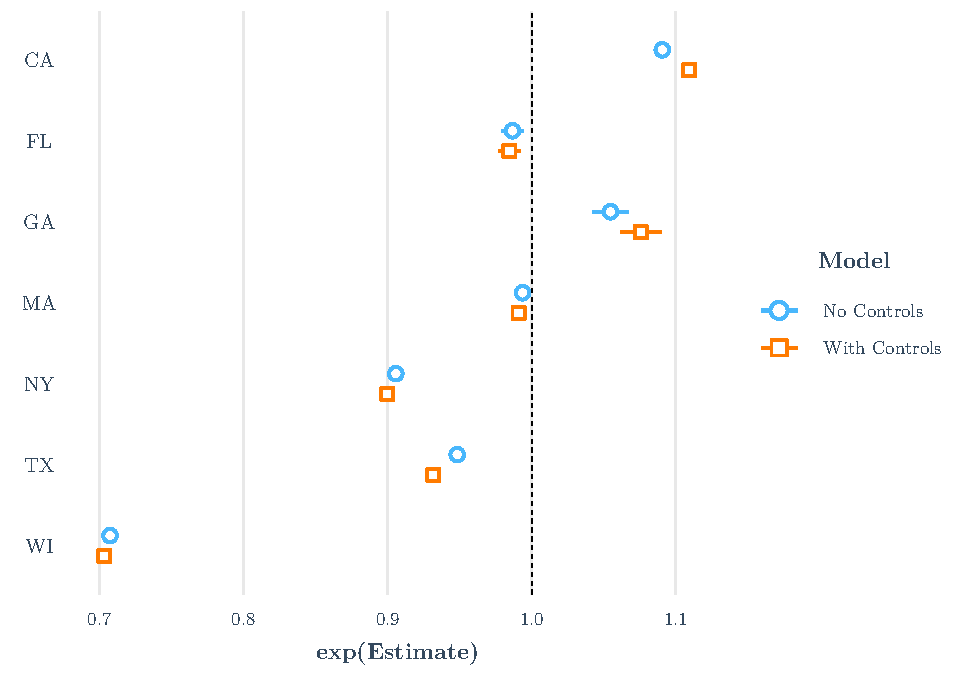
\includegraphics{write_files/figure-latex/overall-plots-1} 

}

\caption{\label{fig:overall-plots}Estimated Effect of Living in Uncontested District for All Voters}\label{fig:overall-plots}
\end{figure}

In each state except California and Georgia, voters who lived in uncontested districts were statistically significantly less likely to turn out than similar voters in other congressional districts. In some states, these effects are surprisingly large: in New York, Texas, and Wisconsin, voters in uncontested districts were at least 5 percentage points less likely to vote than similar voters elsewhere in the state. This is especially surprising in the case of Texas, where a highly-advertised statewide Senate race was waged.

Examining the effects of living in uncontested districts on all voters, however, obscures the differential effect of the treatment on different sorts of voters. In the models below, logistic regressions are run on the subset of treated observations in a given group and their matches, regardless of whether their match shared those characteristics. In other words, if a 39 year old treated voter in California matched with an untreated 40 year old voter, both voters would be included in the ``Younger than 40'' model. If that untreated voter also matched with a 41 year old voter, the untreated voter would also be included in the ``40 to 65'' model.

We begin by examining whether the treatment has a differential effect based on the party affiliation of voters in uncontested districts.\footnote{Although party membership is defined differently in some states that do not have formal party registration, it is uniformly defined \emph{within} each state.} We define ``represented voters'' as individuals who are affiliated with the same party as the unchallenged candidate; ``unrepresented voters,'' then, are individuals affiliated with the opposite party. Figure \ref{fig:party} presents the estimated treatment effect for represented and unrepresented voters in each state.\footnote{In all states but Georgia and Wisconsin, each uncontested race went uncontested by Republicans --- ``Represented Voters'', therefore, are usually Democrats, while ``Unrepresented Voters'' are generally Republicans.}

We find significant differences between the two groups: in four states (California, Florida, Georgia, and Massachusetts), members of the party who ran a candidate were \emph{more} likely to vote than members of that party elsewhere in the state, while members of the unrepresented party were either \emph{less} likely to vote or (in the case of Georiga) turned out at statistically indistinguishable rates from other members of their party. In a fifth state (New York), the treatment effect depressed turnout among represented and unrepresented voters alike, but it had a larger negative effect on opposite party members. It is worth noting that although this relationship is inverted in Texas, our calculation of party affiliation in the Lone Star State is limited to the primary in which a voter participated only in 2018 --- the majority of voters in uncontested races, therefore, have no party affiliation and are dropped from this analysis.

\begin{figure}[H]

{\centering 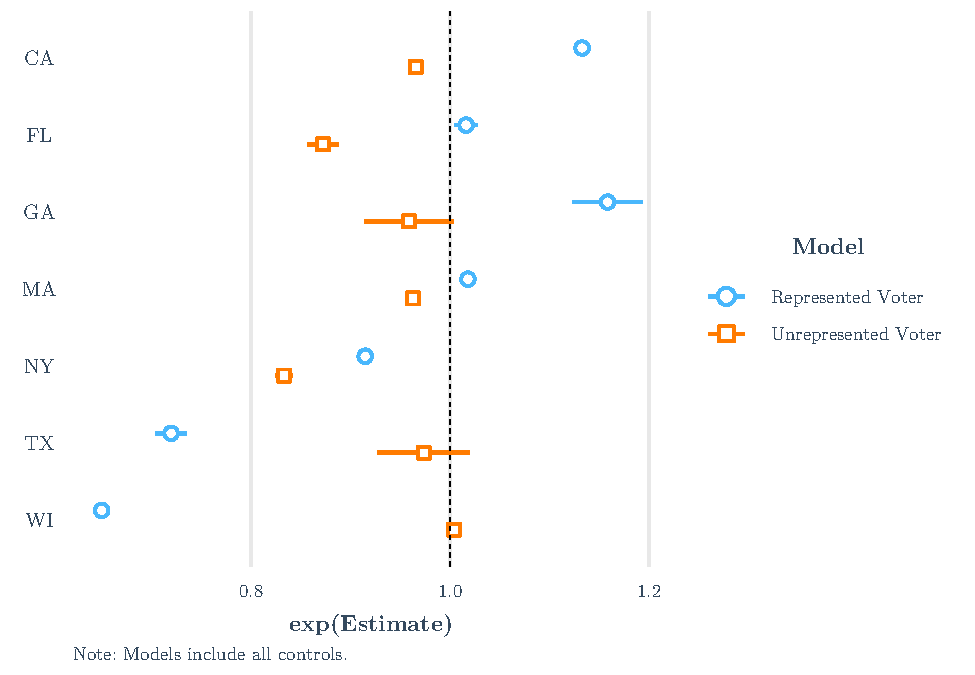
\includegraphics{write_files/figure-latex/party-1} 

}

\caption{\label{fig:party}Estimated Effect of Living in Uncontested District by Party Affiliation}\label{fig:party}
\end{figure}

Women and men similarly responded differently to living in an uncontested district. As Figure \ref{fig:men-women} shows, men were the treatment effect for men was substantially larger than it was for women; in six out of the seven states, the difference was statistically significant. In Florida and Massachusetts, women who lived in uncontested districts were not statistically significantly less likely to vote than women that lived elsewhere --- the negative overall effect, therefore, is driven by men's decreased propensity to vote. In Georgia, where we uncover an overall positive effect of living in an uncontested district, the breakout by gender demonstrates that this is driven by women's increased propensity to participate: men in uncontested districts in Georgia were less likely to vote than men in other parts of the state. Although the treatment is associated with depressed turnout for women in California, New York, and Wisconsin, the treatment effect for women is smaller than for men. The effect size for women in Texas is statistically indistinguishable from that of men.

\begin{figure}[H]

{\centering 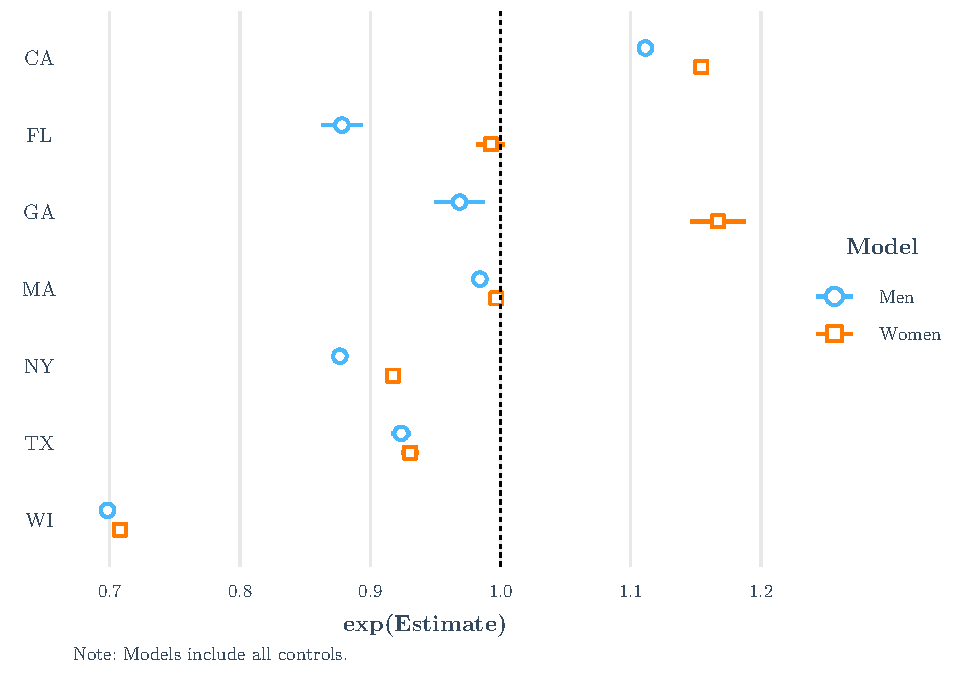
\includegraphics{write_files/figure-latex/men-women-plots-1} 

}

\caption{\label{fig:men-women}Estimated Effect of Living in Uncontested District by Sex}\label{fig:men-women-plots}
\end{figure}

Finally, we break the estimated treatment effects out by voters' age, presented in Figure \ref{fig:age-plots}. Again, we find substantial variation in the estimated effect within most of our study states.\footnote{Because Wisconsin does not track voters' ages, we exclude the state from this analysis.} In four of the six states, young voters in uncontested districts were \emph{more} likely to turn out than their peers elsewhere in the state. In Florida and Massachusetts, this contrasts sharply with the estimated effect on older residents, for whom the treatment effect was negative and significant. In California, where the treatment is associated with an increased propensity to vote for all voters, the effect is much larger for the youngest voters. The positive treatment effect is also much higher for the youngest voters in Georgia than any other age group.

\begin{figure}[H]

{\centering 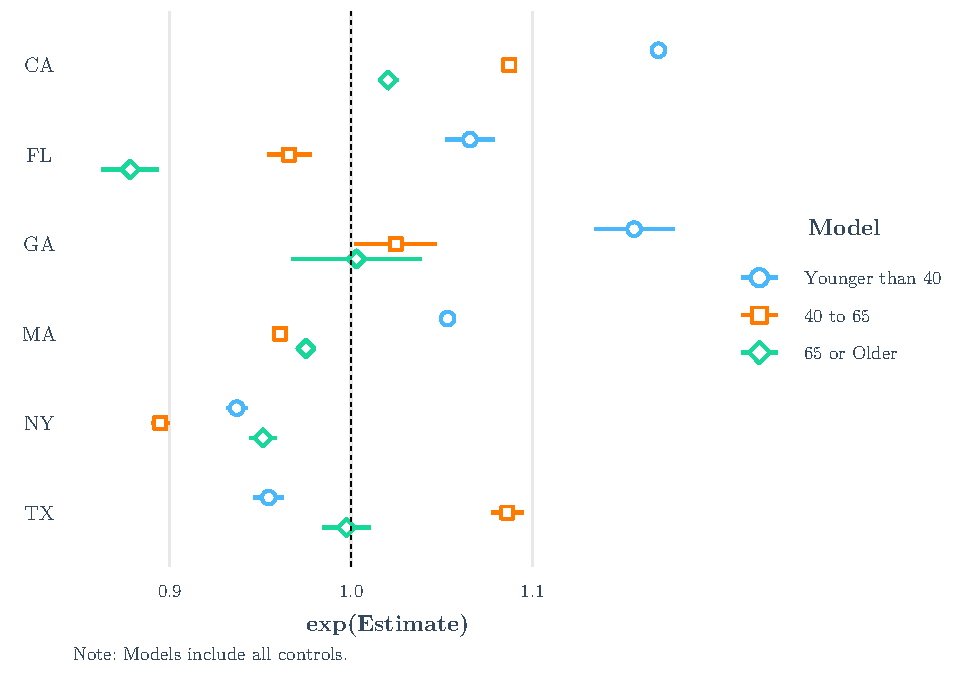
\includegraphics{write_files/figure-latex/age-plots-1} 

}

\caption{\label{fig:ages}Estimated Effect of Living in Uncontested District by Age}\label{fig:age-plots}
\end{figure}

\hypertarget{discussion-and-conclusion}{%
\section*{Discussion and Conclusion}\label{discussion-and-conclusion}}
\addcontentsline{toc}{section}{Discussion and Conclusion}

Our preliminary findings uncover multiple factors at play. We did not expect to find negative treatment effects in any of states studied, and yet voters in uncontested districts in California and Georgia were significantly more likely to vote than similarly situated voters in contested house races. Nevertheless, five of the seven states included in the analysis behaved as expected. In Florida, Massachusetts, New York, Texas, and Wisconsin, voters where a house (or assembly) seat was uncontested voted at significantly lower rates. The magnitude of these decreases was often quite large --- in New York, for instance, voters in uncontested districts were only about 90 percent as likely to cast a ballot as individuals in contested districts. In Wisconsin, the effect was even larger: registered voters in the 37 uncontested districts were just 70 percent as likely to turn out. It appears that the political preferences of uncontested districts are generally as a whole underrepresented in statewide races.

\emph{As a whole}, however, obscures important discrepancies in how voters of different parties respond to treatment. In 4 of the 7 states, voters who affiliated with the party of the unchallenged candidate were \emph{more} likely to participate than similar voters of the same party elsewhere in the state. This increased propensity to vote servely undermines the rational theory of voting. As discussed earlier, under Downs' equation, voters in uncontested districts cannot be more likely to cast a ballot --- and yet, in the 2018 midterm elections, represented voters were more likely to participate.

In New York, Democrats (represented voters) in uncontested districts were less likely to vote than Democrats elsewhere. The treatment effect for Democrats, however, was smaller than for Republicans. In five of seven states, therefore, the treatment effect was significantly larger (that is to say, depressed turnout more) for unrepresented voters than represented voters.\footnote{As discussed above, the party affiliation results for Texas should be taken lightly. Because the current analysis bases party affiliation only off of the primary in which a voter participated in 2018, only 19 percent of Texas voters are assigned to a party. These voters are unlikely to be representative of the whole electorate. The next version of this paper will use data from L2, which models party affiliation based on more historical data.} Although this differential is unexplainable under the rational theory of voting, it is not surprising given the body of scholarship demonstrating that voters who feel their representatives do not reflect their values are less likely to vote. An individual whose party is not even represented on the ballot is likely to feel unrepresented. Although the CCES in 2018 did not ask voters about their perceived efficacy, voters in uncontested districts in 2014 were less likely to report that they believed they were well represented.

As many have noted {[}cite{]}, the 2018 election served in many ways as a referendum on the presidency of Donald Trump. Ballots in 2018, therefore, also carried a highly symbolic value: although Trump was not on the ballot, news stories reported that many individuals cast their ballots to register support or disapproval of the president. It is possible that the symbolic nature of these ballots operated differently in contested than uncontested districts. In uncontested districts, a large majority of the electorate belongs to a single political party. As Mason (\protect\hyperlink{ref-Mason2018}{2018}) and others have demonstrated, voters with few crosscutting identities and few social ties with members of the opposite party are more likely to view politics as a group struggle --- and, perhaps, therefore more likely to ascribe symbolic value to their votes. Voters in uncontested districts are likely to have more (politically) homogenous social networks, which may account for the increased propensity of represented voters to cast a ballot.

The opposite logic may hold true for unrepresented voters in uncontested districts. These voters may be among the \emph{most} likely to have social ties with voters of the other party, simply because so many of their neighbors affiliate with the opposite party. Their relationships with members of the opposite party may engender less intense feelings about Trump (either positive or negative) than members of the same party elsewhere in the state, and may therefore ascribe less symbolic meaning to their ballot. Their (relative) ambivalence toward the Trump Administration, combined with the decrease in ``rationality'' of voting and their decreased feelings of efficacy may all contribute to their depressed turnout.

The consistent difference in treatment effect for men and women is equally surprising. Similarly, the large positive effect for the youngest voters in four out of the six states is puzzling. It is possible that women and younger voters are more impacted by the symbolic nature of the vote, as discussed above, than older voters and men. By the same token, we may simply be picking up the partisan affiliation of these voters: younger voters and women are more likely to be registered Democrats. The vast majority of the represented voters, as defined above, are Democrats. However, these gender and age differences continue to hold even in Georgia, where each major party left one race uncontested. If the gender and age effects were operating merely through an individual's status as an (un)represented voter we would expect these effects to wash one another out in Georgia. This is not the case.

\newpage

\hypertarget{references}{%
\section*{References}\label{references}}
\addcontentsline{toc}{section}{References}

\hypertarget{refs}{}
\begin{cslreferences}
\leavevmode\hypertarget{ref-wapo}{}%
Berkowitz, Bonnie, and Chiqui Esteban. 2018. ``Democrats Lead 40-3 in the House Before Any Votes Are Counted.'' \emph{Washington Post}, October. \url{https://www.washingtonpost.com/graphics/2018/politics/midterms-uncontested-candidates/}.

\leavevmode\hypertarget{ref-Bishop2009}{}%
Bishop, Bill. 2009. \emph{The Big Sort: Why the Clustering of Like-Minded America Is Tearing Us Apart}. Mariner Books.

\leavevmode\hypertarget{ref-Bullock1996}{}%
Bullock, Charles, and Richard Dunn. 1996. ``Election Roll-Off: A Test of Three Explanations.'' \emph{Urban Affairs Review} 32: 71--86.

\leavevmode\hypertarget{ref-Campbell1960}{}%
Campbell, Angus. 1960. ``Surge and Decline: A Study of Electoral Change.'' \emph{Public Opinion Quarterly} 24: 397--418.

\leavevmode\hypertarget{ref-Campbell1991}{}%
Campbell, James. 1991. ``The Presidential Surge and Its Midterm Decline in Congressional Elections, 1868-1988.'' \emph{Journal of Politics} 53: 477--87.

\leavevmode\hypertarget{ref-Fairdosi2015}{}%
Fairdosi, Amir Shawn, and Jon Rogowski. 2015. ``Candidate Race, Partisanship, and Political Participation: When Do Black Candidates Increase Black Turnout?'' \emph{Political Research Quarterly} 68: 337--49.

\leavevmode\hypertarget{ref-Fraga2016}{}%
Fraga, Bernard. 2016. ``Redistricting and the Causal Impact of Race on Voter Turnout.'' \emph{Journal of Politics} 78: 19--34.

\leavevmode\hypertarget{ref-Griffin2006}{}%
Griffin, John, and Michael Keane. 2006. ``Descriptive Representation and the Composition of African American Turnout.'' \emph{American Journal of Political Science} 50: 998--1012.

\leavevmode\hypertarget{ref-Hall1987}{}%
Hall, William, and Larry Aspin. 1987. ``The Roll-Off Effect in Judicial Retention Elections.'' \emph{Social Science Journal} 24: 415--27.

\leavevmode\hypertarget{ref-Hayes2009}{}%
Hayes, Danny, and Seth McKee. 2009. ``The Participatory Effects of Redistricting.'' \emph{American Journal of Political Science} 53: 1006--23.

\leavevmode\hypertarget{ref-Hood2010}{}%
Hood, M. V., and Seth McKee. 2010. ``Stranger Danger: Redistricting, Incumbent Recognition, and Vote Choice.'' \emph{Social Science Quarterly} 91: 344--58.

\leavevmode\hypertarget{ref-Imai2016}{}%
Imai, Kosuke, and Kabir Khanna. 2016. ``Improving Ecological Inference by Predicting Individual Ethnicity from Voter Registration Records.'' \emph{Political Analysis} 24 (2): 263--72. \url{https://doi.org/10.1093/pan/mpw001}.

\leavevmode\hypertarget{ref-Knack2003}{}%
Knack, Stephen, and Martha Kropf. 2003. ``Roll-Off at the Top of the Ballot: Intentional Undervoting in American Presidential Elections.'' \emph{Politics and Policy} 31: 575--94.

\leavevmode\hypertarget{ref-Konisky2011}{}%
Konisky, David, and Michiko Ueda. 2011. ``The Effects of Uncontested Elections on Legislator Performance.'' \emph{Legislative Studies Quarterly} 36: 199--229.

\leavevmode\hypertarget{ref-Levitt1997}{}%
Levitt, Steven, and Catherine Wolfram. 1997. ``Decomposing the Sources of Incumbency Advantage in the U.s. House.'' \emph{Legislative Studies Quarterly} 22: 45--60.

\leavevmode\hypertarget{ref-Mason2018}{}%
Mason, Lilliana. 2018. \emph{Uncivil Agreement}. The University of Chicago Press. \url{https://www.ebook.de/de/product/29988704/lilliana_mason_uncivil_agreement.html}.

\leavevmode\hypertarget{ref-McKee2008}{}%
McKee, Seth. 2008. ``Redistricting and Familiarity with U.s. House Candidates.'' \emph{American Politics Research} 36: 962--79.

\leavevmode\hypertarget{ref-Reilly2009}{}%
Reilly, Shauna, and Sean Richey. 2009. ``Ballot Question Readability and Roll-Off: The Impact of Language Complexity.'' \emph{Political Research Quarterly} 64: 59--67.

\leavevmode\hypertarget{ref-Sekhon2011}{}%
Sekhon, Jasjeet S. 2011. ``Multivariate and Propensity Score Matching Software with Automated Balance Optimization: TheMatchingPackage forR.'' \emph{Journal of Statistical Software} 42 (7). \url{https://doi.org/10.18637/jss.v042.i07}.

\leavevmode\hypertarget{ref-Squire1989}{}%
Squire, Peverill. 1989. ``Competition and Uncontested Seats in U.s. House Elections.'' \emph{Legislative Studies Quarterly} 14: 281--95.

\leavevmode\hypertarget{ref-Wattenberg2000}{}%
Wattenberg, Martin, Ian McAllister, and Anthony Salvanto. 2000. ``How Voting Is Like Taking an Sat Test: An Analysis of American Voter Rolloff.'' \emph{American Politics Research} 28: 234--50.

\leavevmode\hypertarget{ref-Wielhouwer1994}{}%
Wielhouwer, Peter, and Brad Lockerbie. 1994. ``Party Contacting and Political Participation, 1952-90.'' \emph{American Journal of Political Science} 38: 211--29.

\leavevmode\hypertarget{ref-Winburn2009}{}%
Winburn, Jonathan, and Michael Wagner. 2009. ``Carving Voters Out: Redistricting's Influence on Political Information, Turnout, and Voting Behavior.'' \emph{Political Research Quarterly} 63: 373--86.

\leavevmode\hypertarget{ref-Wrighton1997}{}%
Wrighton, Mark, J, and Peverill Squire. 1997. ``Uncontested Seats and Electoral Competition for the U.s. House of Representatives over Time.'' \emph{Journal of Politics} 59: 452--68.

\leavevmode\hypertarget{ref-Yoshinaka2009}{}%
Yoshinaka, Antoine, and Chad Murphy. 2009. ``Partisan Gerrymandering and Population Instability: Completing the Redistricting Puzzle.'' \emph{Political Geography} 28: 451--62.
\end{cslreferences}

\end{document}
